% ==================================================
% ① 基本設定・パッケージの読み込み
% ==================================================
\documentclass[unicode,10pt]{beamer}
\usepackage{luatexja} % LuaLaTeXで日本語を使うための必須パッケージ
\usetheme{metropolis} % モダンなデザインのテーマ
\usepackage{amsmath, amssymb, amsthm} % 数式・数学記号用
\usepackage{bussproofs} % 自然演繹などの証明図を描画するためのパッケージ
\usepackage{tikz} % 図形描画用（フッターの三角形などに使用）
\usepackage{luatexja-fontspec} % LuaLaTeXでのフォント設定用

% ==================================================
% ② カラー・フォントの設定
% ==================================================
\definecolor{mygray}{gray}{0.9} % カスタムカラー（薄い灰色）の定義
\setsansfont{Arial} % 欧文の基本フォントをArialに指定
\usefonttheme{serif} % 数式や一部の英字をセリフ体（明朝体系）にして読みやすくする

% ==================================================
% ③ スライドのレイアウト・デザイン設定
% ==================================================
\setbeamertemplate{navigation symbols}{} % ナビゲーションアイコンを非表示

% --- ヘッダーのカスタマイズ ---
\setbeamertemplate{headline}{%
  \leavevmode%
  \setbeamercolor{hbox_color}{fg=black, bg=mygray}%
  \begin{beamercolorbox}[wd=\paperwidth, ht=11ex, dp=0ex, right, sep=0ex]{hbox_color}%
    \includegraphics[height=11ex]{docs/logo.png}%
  \end{beamercolorbox}%
}

% --- フッターのカスタマイズ ---
\setbeamertemplate{footline}{%
  \leavevmode%
  \begin{beamercolorbox}[wd=\paperwidth, ht=4ex, dp=2ex, right]{}%
    \begin{tikzpicture}[remember picture, overlay]
      \fill[mygray] (current page.south east) -- ++(-1.2,0) -- ++(1.2,1.2) -- cycle;
      \node[anchor=south east, xshift=-0.5ex, yshift=0.5ex] at (current page.south east) {%
        \usebeamerfont{page number in head/foot}\insertframenumber{} / \inserttotalframenumber%
      };
    \end{tikzpicture}%
  \end{beamercolorbox}%
}

% --- ページタイトルの位置調整 ---
\setbeamertemplate{frametitle}{%
  \vspace{2ex}%
  \begin{beamercolorbox}[wd=\paperwidth, left]{frametitle}%
    \hspace{2ex}\usebeamerfont{frametitle}\insertframetitle% 
  \end{beamercolorbox}%
  \vspace{-1ex}%
}
\setbeamercolor{frametitle}{fg=black, bg=} % タイトルの色を黒に固定

% ==================================================
% ④ タイトルページの情報
% ==================================================
\title{Logic and Structure 輪読}
\subtitle{第1章：命題論理}
\author{発表者：あなたの名前}
\date{\today}

% ==================================================
% ⑤ ここから下がスライドの本文（コンテンツ）です
% ==================================================
\begin{document}

\begin{frame}[plain]
    \titlepage
\end{frame}

% ==============================
% テンプレート集：使い方のサンプル
% ==============================
\section{TeXスライドの基本（テンプレート集）}

\begin{frame}[fragile]{数式と定理環境 (amsmath, amssymb, amsthm)}
    \textbf{複数行の数式（align環境）：}
    等号（$\equiv$）の位置を \verb|&| で揃えて綺麗に表示します。
    \begin{align*}
        (A \lor B) \land C &\equiv (A \land C) \lor (B \land C) \\
        \neg(A \land B) &\equiv \neg A \lor \neg B
    \end{align*}

    \textbf{数学・論理記号（amssymb）：}
    自然数 $\mathbb{N}$、実数 $\mathbb{R}$、空集合 $\emptyset$ や $\varnothing$

    \vspace{1em}
    \textbf{定理環境（amsthm / Beamer標準機能）：}
    \begin{theorem}[ド・モルガンの法則]
        任意の命題 $A, B$ について、$\neg(A \lor B) \equiv \neg A \land \neg B$ が成り立つ。
    \end{theorem}
\end{frame}

\begin{frame}[fragile]{証明図の描画 (bussproofs)}
    自然演繹などの推論の木構造を簡単に描けます。

    \vspace{1em}
    \begin{center}
    \begin{prooftree}
        \AxiomC{$\phi \to \psi$} % 1つ目の前提
        \AxiomC{$\phi$}          % 2つ目の前提
        \RightLabel{$(\to E)$}   % 推論規則のラベルを右に添える
        \BinaryInfC{$\psi$}      % 2つの前提から線を引いて結論を出す
    \end{prooftree}
    \end{center}
    \vspace{1em}

    \textbf{主なコマンド：}
    \begin{itemize}
        \item \verb|\AxiomC{...}| : 前提（公理）を上に配置
        \item \verb|\UnaryInfC{...}| : 1つの前提から推論（1本線）
        \item \verb|\BinaryInfC{...}| : 2つの前提から推論
        \item \verb|\RightLabel{...}| : 引いた線の右側に文字を添える
    \end{itemize}
\end{frame}

\begin{frame}[fragile]{図形の描画 (tikz)}
    スライド内にクリプキモデルなどのグラフや図形を直接描画できます。

    \begin{center}
    % node distanceでノード間の基本距離を設定
    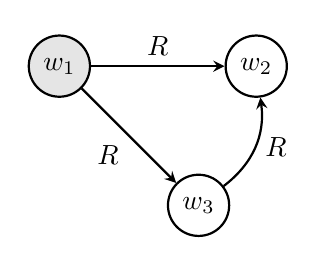
\begin{tikzpicture}[node distance=2.5cm, thick]
        % ノード（状態・世界）の定義
        \node[circle, draw, fill=mygray] (W1) {$w_1$};
        \node[circle, draw, right of=W1] (W2) {$w_2$};
        \node[circle, draw, below right of=W1] (W3) {$w_3$};

        % 矢印（関係性）の描画
        \draw[->, >=stealth] (W1) -- node[above] {$R$} (W2);
        \draw[->, >=stealth] (W1) -- node[below left] {$R$} (W3);
        \draw[->, >=stealth] (W3) to [bend right=30] node[right] {$R$} (W2);
    \end{tikzpicture}
    \end{center}

    \textbf{主なコマンド：}
    \begin{itemize}
        \item \verb|\node| : 丸や四角などの要素（頂点）を配置します。
        \item \verb|\draw[->]| : 頂点同士を矢印（エッジ）で結びます。\verb|bend| オプションで矢印を曲げることも可能です。
    \end{itemize}
\end{frame}

% ==============================
% 実際のスライド例（本編）
% ==============================
\section{本編スライド例}

\begin{frame}{1-1. 命題論理の定義}
    命題論理の定義は以下の通りです。
    \begin{itemize}
        \item \textbf{命題}：真または偽の値を持つ文
        \item \textbf{論理結合子}：$\land$（かつ）、$\lor$（または）、$\rightarrow$（ならば）、$\neg$（否定）など
        \item \textbf{真理値表}：各命題の真偽値を示す表
    \end{itemize}
\end{frame}

\end{document}